\section{Method}\label{sec:method}
In order to process the accelerometer and TAC value timeseries data, an approach dealing with the continuous data stream over time is required.
Since almost all machine learning approaches require an input of constant length, a technique such as the sliding window time series analysis, combined with sequence padding, can be used.
This method enables the analysis on fractions of the time series data with a constant length.
The sliding window therefore partitions the data into a number of finite-length segments and tries to relate $ws$ past data points to a prediction $y$ by grouping \cite{MOZAFFARI2015150}.
The sliding window is defined by the parameters windows size ($ws$) and the stride size ($ss$).
So at any given point $t_n$ in time $t$, the subset tuple 

\begin{equation}
	s_{t_n} = (\{ x_{t_{n - i}}, x \in X, ws > i \geq 0 \}, y_{t_n})
\end{equation}

is calculated.
As all data points are evenly spaced out due to the resampling, we do not have to take the elapsed time between observations into account.
The stride indicates the increment of $n$ for $t_n$.
For this regression, a window size of $10\si{\second}$ and a stride of $2\si{\second}$ was used.
The window size was chosen as in \cite{DBLP:conf/ijcai/KillianPNMC19} and the stride values were determined experimentally in order to create a feasible amount of data to work with that could still represent motion and does lack specific scientific justification.
















\subsection{Feature Extraction}\label{ssec:feature}
By applying the sliding window with the parameters as stated above on the data resampled at $40 \si{\hertz}$, this results in a feature matrix of $400 \times 3$ features. In order to reduce the amount of data and increase the information at the same time, a manual feature extraction phase was implemented.
The extracted features are shown in table \ref{tab:features}. Principal component analysis (PCA) is used for dimensionality reduction to avoid issues like overfitting. The three-dimensional accelerometer data is reduced into one dimension by using the PCA class from  \texttt{scikit-learn} \cite{scikit-learn}.

\begin{table}[h]
	\resizebox{\columnwidth}{!}{%
		\centering
		\begin{tabular}{|l|c|l|}
			\hline
			Features & Generated data & Definition\\
			\hline
			
			First & 3 & The first elements per axis\\
			Last & 3 & The last elements per axis\\
			Mean & 3 & The mean per axis\\
			Median & 3 & The median per axis\\
			Var & 3 & The variation per axis\\
			Std & 3 & The standard deviation per axis\\
			Min & 3 & The minimum per axis\\
			Max & 3 & The maximum per axis\\
			Argmin & 3 & The index of the minimum per axis\\
			Argmax & 3 & The index of the maximum per axis\\
			Sum & 3 & The sum per axis\\
			Q50 & 3 & The 50\% quantile per axis\\
			Q75 & 3 & The 75\% quantile per axis\\
			Q25 & 3 & The 25\% quantile per axis\\
			PCA & 400 & The principal component value of all 3 axis\\
			MinPCA & 1 & The minimum of PCA\\
			MaxPCA & 1 & The maximum of PCA\\
			MeanPCA & 1 & The mean of PCA\\
			
			
			\hline
		\end{tabular}
	}
	\caption{Features extracted per sliding window dataframe.}
	\label{tab:features}
\end{table}

Additional parameters have been extracted using \texttt{tsfresh} \cite{DBLP:journals/ijon/ChristBNK18}, but not all algorithms have been trained with the additional features due to runtime constraints.

\begin{table}[h]
	\resizebox{\columnwidth}{!}{%
		\centering
		\begin{tabular}{|l|c|l|}
			\hline
			Features & Generated data & Description \\
			\hline
			
			abs\_energy & 3 & \href{https://tsfresh.readthedocs.io/en/latest/api/tsfresh.feature_extraction.html\#tsfresh.feature_extraction.feature_calculators.abs_energy}{absenergy per axis}\\
			absolute sum of changes & 3 & \href{https://tsfresh.readthedocs.io/en/latest/api/tsfresh.feature_extraction.html\#tsfresh.feature_extraction.feature_calculators.abs_energy}{absolute sum of changes per axis}\\
			autocorrelation & 3 & \href{https://tsfresh.readthedocs.io/en/latest/api/tsfresh.feature_extraction.html\#tsfresh.feature_extraction.feature_calculators.autocorrelation}{autocorrelation per axis}\\
			binned\_entropy & 3 & \href{https://tsfresh.readthedocs.io/en/latest/api/tsfresh.feature_extraction.html\#tsfresh.feature_extraction.feature_calculators.binned_entropy}{binned entropy per axis}\\
			c3 & 3 & \href{https://tsfresh.readthedocs.io/en/latest/api/tsfresh.feature_extraction.html\#tsfresh.feature_extraction.feature_calculators.c3}{c3 per axis}\\
			cid\_ce & 3 & \href{https://tsfresh.readthedocs.io/en/latest/api/tsfresh.feature_extraction.html\#tsfresh.feature_extraction.feature_calculators.cid_ce}{cid ce per axis}\\
			count\_above & 3 & \href{https://tsfresh.readthedocs.io/en/latest/api/tsfresh.feature_extraction.html\#tsfresh.feature_extraction.feature_calculators.count_above}{count above per axis}\\
			count\_above\_mean & 3 & \href{https://tsfresh.readthedocs.io/en/latest/api/tsfresh.feature_extraction.html\#tsfresh.feature_extraction.feature_calculators.count_above_mean}{count above mean per axis}\\
			count\_below & 3 & \href{https://tsfresh.readthedocs.io/en/latest/api/tsfresh.feature_extraction.html\#tsfresh.feature_extraction.feature_calculators.count_below}{count below per axis}\\
			count\_below\_mean & 3 & \href{https://tsfresh.readthedocs.io/en/latest/api/tsfresh.feature_extraction.html\#tsfresh.feature_extraction.feature_calculators.count_below_mean}{count below mean per axis}\\
			first\_location\_of\_maximum & 3 & \href{https://tsfresh.readthedocs.io/en/latest/api/tsfresh.feature_extraction.html\#tsfresh.feature_extraction.feature_calculators.first_location_of_maximum}{first location of maximum per axis}\\
			first\_location\_of\_minimum & 3 & \href{https://tsfresh.readthedocs.io/en/latest/api/tsfresh.feature_extraction.html\#tsfresh.feature_extraction.feature_calculators.first_location_of_minimum}{first location of minimum per axis}\\
			kurtosis & 3 & \href{https://tsfresh.readthedocs.io/en/latest/api/tsfresh.feature_extraction.html\#tsfresh.feature_extraction.feature_calculators.kurtosis}{kurtosis per axis}\\
			last\_location\_of\_maximum & 3 & \href{https://tsfresh.readthedocs.io/en/latest/api/tsfresh.feature_extraction.html\#tsfresh.feature_extraction.feature_calculators.last_location_of_maximum}{last location of maximum per axis}\\
			last\_location\_of\_minimum & 3 & \href{https://tsfresh.readthedocs.io/en/latest/api/tsfresh.feature_extraction.html\#tsfresh.feature_extraction.feature_calculators.last_location_of_minimum}{last location of minimum per axis}\\
			longest\_strike\_above\_mean & 3 & \href{https://tsfresh.readthedocs.io/en/latest/api/tsfresh.feature_extraction.html\#tsfresh.feature_extraction.feature_calculators.longest_strike_above_mean}{longest strike above mean per axis}\\
			longest\_strike\_below\_mean & 3 & \href{https://tsfresh.readthedocs.io/en/latest/api/tsfresh.feature_extraction.html\#tsfresh.feature_extraction.feature_calculators.longest_strike_below_mean}{longest strike below mean per axis}\\
			mean\_abs\_change & 3 & \href{https://tsfresh.readthedocs.io/en/latest/api/tsfresh.feature_extraction.html\#tsfresh.feature_extraction.feature_calculators.mean_abs_change}{mean abs change per axis}\\
			mean\_change & 3 & \href{https://tsfresh.readthedocs.io/en/latest/api/tsfresh.feature_extraction.html\#tsfresh.feature_extraction.feature_calculators.mean_change}{mean change per axis}\\
			mean\_second\_derivative\_central & 3 & \href{https://tsfresh.readthedocs.io/en/latest/api/tsfresh.feature_extraction.html\#tsfresh.feature_extraction.feature_calculators.mean_second_derivative_central}{mean second derivative central per axis}\\
			number\_crossing m & 3 & \href{https://tsfresh.readthedocs.io/en/latest/api/tsfresh.feature_extraction.html\#tsfresh.feature_extraction.feature_calculators.number_crossing_m}{number crossing m per axis}\\
			number\_peaks & 3 & \href{https://tsfresh.readthedocs.io/en/latest/api/tsfresh.feature_extraction.html\#tsfresh.feature_extraction.feature_calculators.number_peaks}{number peaks per axis}\\
			skewness & 3 & \href{https://tsfresh.readthedocs.io/en/latest/api/tsfresh.feature_extraction.html\#tsfresh.feature_extraction.feature_calculators.skewness}{skewness per axis}\\
			time\_reversal\_asymmetry\_statistic & 3 & \href{https://tsfresh.readthedocs.io/en/latest/api/tsfresh.feature_extraction.html\#tsfresh.feature_extraction.feature_calculators.time_reversal_asymmetry_statistic}{time reversal asymmetry statistic per axis}\\
			variation\_coefficient & 3 & \href{https://tsfresh.readthedocs.io/en/latest/api/tsfresh.feature_extraction.html\#tsfresh.feature_extraction.feature_calculators.variation_coefficient}{variation coefficient per axis}\\
			\hline
		\end{tabular}
	}

	\caption{Additional features extracted using \texttt{tsfresh} \cite{DBLP:journals/ijon/ChristBNK18}.}
	\label{tab:features-additional}
\end{table}



In comparison to \cite{DBLP:conf/ijcai/KillianPNMC19}, a few things are handled differently already: first, all of the above features are calculated on the whole window, while \citeauthor{DBLP:conf/ijcai/KillianPNMC19} used a two-tiered window approach, a short-term and a long-term window, and some additional features, that were calculated separately \cite{DBLP:conf/ijcai/KillianPNMC19}.
Secondly, \citeauthor{DBLP:conf/ijcai/KillianPNMC19} extracted features more specific to audio analysis.
Their features sum up to $1215$ data points, while we currently extract $445$ with $72$ additional \texttt{tsfresh} features, creating a total of $517$. 
This already shows a significant difference between the methods used and introduces additional obstacles for comparison.














\subsection{Hyperparameter Optimization}\label{ssec:hpo}
In order to create the best possible regressor, another important element besides feature extraction is the tuning of said model. 
While parameters are learned during training – for example the slope of linear regression or weights of neural network, hyperparameters can be arbitrarily set by a data scientist beforehand.



\begin{figure}[h]
	\centering
	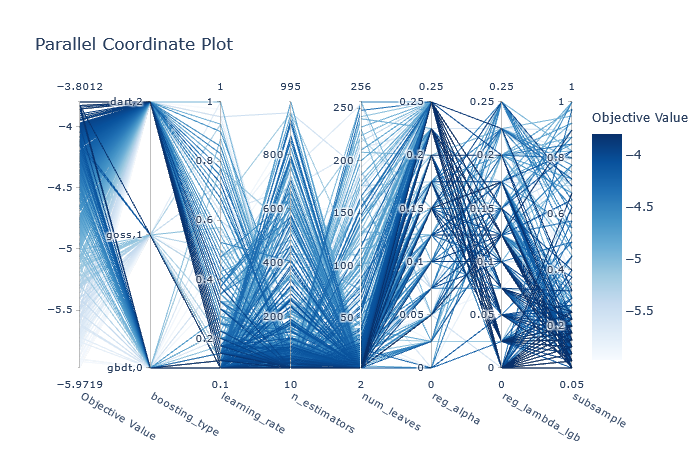
\includegraphics[width=\columnwidth]{hpo-parallel}
	\caption{Exemplary HPO value plot for \texttt{LightGBM} with sample \texttt{JB3156} chunk 0}
	\label{fig:hpo-parallel}
\end{figure}



Therefore, the selection of correct values for these hyperparameters is crucial and can significantly improve the performance of a model.
This tuning process can be viewed as a type of optimization problem itself cause we aim to find the right combination of a set of hyperparameters to e.g. minimize the loss or maximize the performance metric.
Apart from a manual search, random search and grid search are viable options.
However, such an approach is more or less equal to a brute force attempt.
Hence, so called automated hyperparameter optimization (HPO) algorithms have evolved, using techniques such as bayesian optimization, gradient descent and evolutionary algorithms.
This enables efficiently searching large spaces and pruning of unpromising trials for faster results.


Multiple libraries can be used; most famous contenders \texttt{Hyperopt} \cite{DBLP:conf/icml/BergstraYC13} and \texttt{Optuna} \cite{DBLP:conf/kdd/AkibaSYOK19} are subject of countless articles comparing them (e.g. \cite{neptune_2019}). \texttt{Optuna} was chosen based on the better documentation and build-in visualization.


A hyperparameter optimization study was performed separately for each of the algorithms presented in \ref{ssec:algorithms}.
Figure \ref{fig:hpo-parallel} shows a value plot for different hyperparameters for the \texttt{LightGBM} \cite{DBLP:conf/nips/KeMFWCMYL17} algorithm, validated the chunk number $0$ of sample \texttt{JB3156}.
This dataset was chosen because it is the largest file after splitting.

Depending on the runtime of the algorithm and the respective features, each study was optimized for $100 - 1000$ trials.


\begin{figure*}[bt]
	\centering
	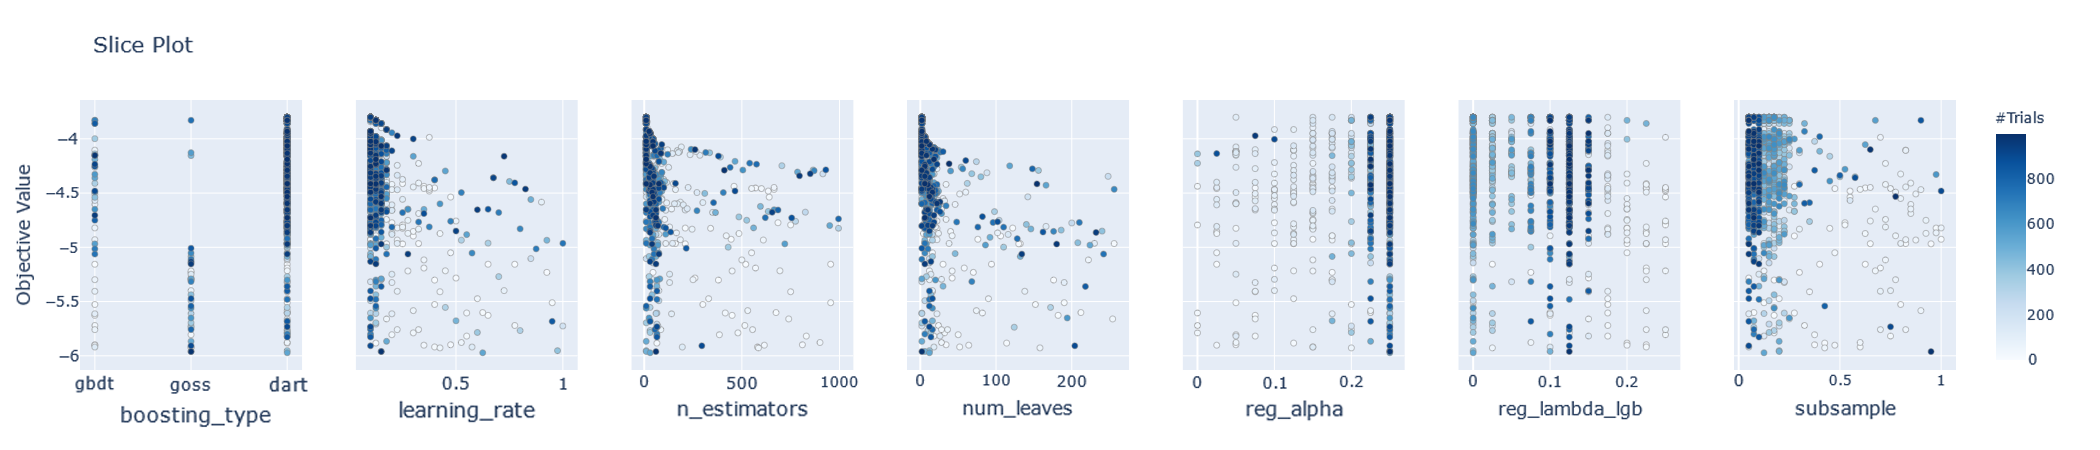
\includegraphics[width=\textwidth]{hpo-sliceBIG}
	\caption{Exemplary HPO slice plot for \texttt{LightGBM} with sample \texttt{JB3156} chunk 0}
	\label{fig:hpo-slice}
\end{figure*}

\begin{figure}[h]
	\centering
	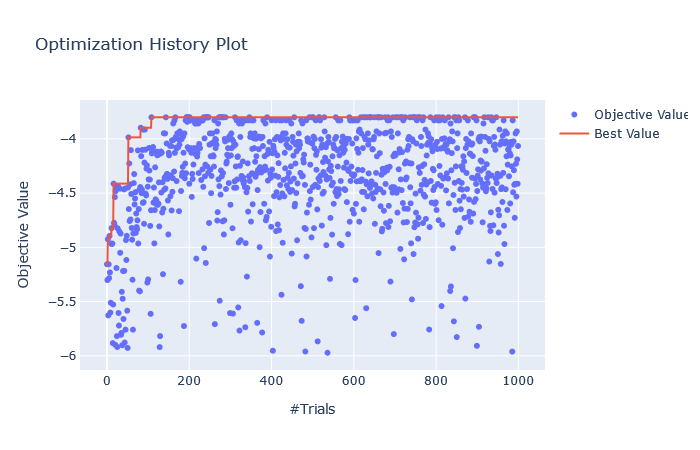
\includegraphics[width=\columnwidth]{hpo-hist}
	\caption{Exemplary HPO history plot for \texttt{LightGBM} with sample \texttt{JB3156} chunk 0}
	\label{fig:hpo-hist}
\end{figure}

Figure \ref{fig:hpo-slice} shows the variation of each hyperparameter over time.
Whereas the final optimization history is shown in figure \ref{fig:hpo-hist}.
This graph already clearly indicates, that the optimization reached a plateau quite fast and was unable to significantly improve the performance further on.
In case that this model can not satisfy the desired performance requirements, further work in \ref{ssec:feature} is needed.










\subsection{Algorithms}\label{ssec:algorithms}
In ensemble learning theory, we call weak learners (or base models) models that can be used as building blocks for designing more complex models by combining several of them.
Most of the time, these basics models perform not so well by themselves either because they have a high bias often due to low degree of freedom models or because they have too much variance to be robust in case of high degree of freedom models.
But a low bias and a low variance, although they most often vary in opposite directions, are the two most fundamental features expected for a model. 
This is the well known bias-variance tradeoff.

So the idea of ensemble methods is to try reducing bias and/or variance of such weak learners by combining several of them together in order to create a strong learner (or ensemble model) that achieves better performances than any algorithm alone.
One can combine these models in different ways; three major kinds are known in literature: bagging to decrease the model’s variance, boosting decreasing the model’s bias, and stacking to increasing the predictive force of the classifier.

Thus, in consideration of our research question, the algorithms used all implement the concept of ensemble learning.
We evaluated \texttt{ExtraTrees}, \texttt{RandomForest}, \texttt{AdaBoost}, \texttt{GradientBoosting}, and \texttt{HistGradientBoosting} from the popular \texttt{scikit-learn} library \cite{scikit-learn} to establish a baseline for better comparison.

Nonetheless, one of the most popular shallow learning techniques in recent years has been gradient boosting, dominating many Kaggle (subsidiary of Google LLC, online community of data scientists and machine learning practitioners) competitions with heterogeneous tabular data.
Similar to random forest, gradient boosting works by ensembling many decision trees in order to perform regression or classification.
However, unlike random forest, gradient boosting grows trees sequentially, iteratively growing trees based on the residuals of the previous tree.
Doing so allows gradient boosting to focus on particularly tricky observations and yields an extraordinarily powerful ensemble of trees.
Among the most common algorithms in recent years are \texttt{XGBoost} \cite{DBLP:conf/kdd/ChenG16}, \texttt{LightGBM} \cite{DBLP:conf/nips/KeMFWCMYL17} and \texttt{CatBoost} \cite{DBLP:journals/corr/abs-1810-11363}.

All used algorithms share an implementation of the \texttt{scikit-learn} API \cite{sklearn_api}, which made it easy to use a shared infrastructure.
